\documentclass{article}
\usepackage{blindtext}
\usepackage{titlesec}

\usepackage{amsmath, amsfonts}

\usepackage{graphicx}
\usepackage{float}

\title{Lecture Summary: Machine Learning}
\author{Robin Schmitt}

\DeclareMathOperator*{\E}{\mathbb{E}}

\renewcommand{\emph}[1]{\textbf{#1}}

\graphicspath{{figs/}}


\begin{document}

\maketitle

\tableofcontents

\section{Probability Theory}

Two random variables $X$ and $Y$.

\begin{itemize}
  \item Joint probability: $p(X, Y)$
  \item Marginal probability: $p(X)$
  \item Conditional probability: $p(X|Y)$
  \item Sum rule: $p(X) = \sum_{j=1}^L p(X, Y)$
  \item Product rule: $p(X, Y) = p(Y|X)p(X)$
  \item Bayes' theorem: $p(Y|X) = \frac{p(X|Y)p(Y)}{p(X)}$
  \item probability density function: $p(x \in (a,b)) = \int_a^b p(x) dx$
  \item probability density function: $P(z) = \int_{-\infty}^z p(x) dx$
  \item expectation: average value of some function $f(x)$ under some probability distribution $p(x)$
  \item variance: variability around mean value: $\text{var}(f) = \E \left [ (f(x) - \E[f(x)])^2 \right ]$
  \item covariance of two random variables: $\text{cov}(x,y) = \E_{x,y} [(x-\E[x])(y-\E[y])]$
  \begin{itemize}
    \item if $x$ and $y$ are vectors, the result is a covariance matrix
  \end{itemize}
\end{itemize}

\section{Bayes' Decision Theory}

\begin{itemize}
  \item priors: what we can tell about the probability before seeing the data
  \item likelihood: $p(x|C_k)$ describes the likelihood for class $C_k$

  \begin{figure}[H]
    \centering
    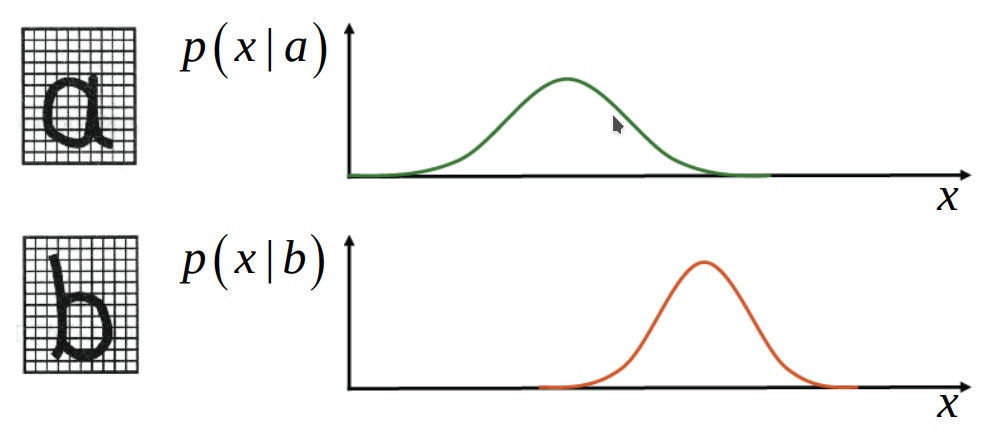
\includegraphics[width=.5\textwidth]{bayes_likelihood1.png}
  \end{figure}

  \begin{itemize}
    \item choose class with higher likelihood
  \end{itemize}

  \item posterior (Bayes' Theorem): $p(C_k|x) = \frac{p(x|C_k)p(C_k)}{p(x)}$
  \item minimize misclassification probability

  \begin{figure}[H]
    \centering
    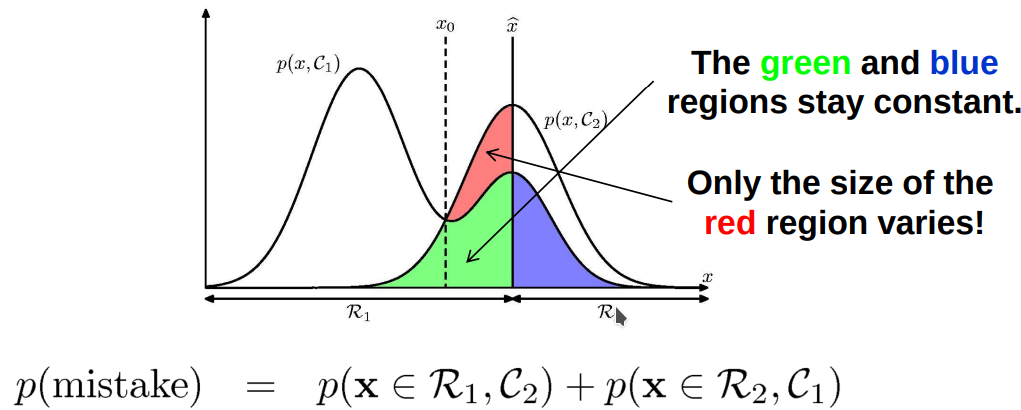
\includegraphics[width=.5\textwidth]{bayes_misclassification}
  \end{figure}

  \item optimal decision rule: decide for class $k$ if
  \begin{align*}
    p(C_k|c) &> p(C_j|x) \quad \forall j \not = k \\
    p(x|C_k)p(C_k) &> p(x|C_j)p(C_j) \quad \forall j \not = k \\
    \frac{p(x|C_k)}{p(x|C_j)} &> \frac{p(C_j)}{p(C_k)} \quad \forall j \not = k \quad \text{(likelihood-ratio test)}
  \end{align*}

  \item introduce \emph{loss function} for classification \[
    L_{kj} = \text{loss for decision $C_j$ if truth is $C_k$}
  \]
  \begin{itemize}
    \item true class is unknown $\Rightarrow$ minimize expected loss $\Rightarrow$ choose regions $R_j$ such that \[
      \E[L] = \sum_k L_{kj} p(C_k | x)
    \]
    is minimized
  \end{itemize}
  \item reject decision, if largest posterior is significantly smaller than 1
  \end{itemize}

  \subsection{Discriminant Functions}

  Given discriminant functions $y_1(x), ..., y_K(x)$, classify $x$ as class $C_k$ if \[
    y_k(x) > y_j(x) \forall j \not = k.
  \]

  \begin{itemize}
    \item generative methods: $y_k(x) \propto p(x|C_k)p(C_k)$
    \item discriminative methods: $y_k(x) \propto p(C_k|x)$
  \end{itemize}

\section{Probability Density Estimation}

\begin{itemize}
  \item supervised learning: data and class labels are known
  \item estimate densities for each class $C_k$ separately: $p(x|C_k)$
\end{itemize}

\subsection{Gaussian Distribution}

\begin{itemize}
  \item one-dimensional case: \[
    \mathcal{N}(x|\mu, \sigma^2) = \frac{1}{\sqrt{2\pi}\sigma} \exp \left \{ - \frac{(x-\mu)^2}{2\sigma^2} \right \}
  \]
  \item multi-dimensional case: \[
    \mathcal{N}(x|\mu, \Sigma) = \frac{1}{(2\pi)^{D/2}|\Sigma|^{1/2}} \exp \left \{
      - \frac{1}{2} (x-\mu)^\top \Sigma^{-1}(x-\mu) \right \}
  \]
  \item \emph{Central limit theorem}: the distribution of the sum of $N$ i.i.d. random variables becomes increasingly Gaussian as $N$ grows.
  \item exponent of $\mathcal{N}$ is called \emph{Mahalanobis distance} \[
    \Delta^2 = (x-\mu)^\top \Sigma^{-1}(x-\mu)
  \]
  \item Slides 3, page 21
\end{itemize}

\subsection{Parametric Representations}

\begin{itemize}
  \item learn, by estimating parameters $\theta$ of distribution
  \item likelihood of $\theta$: $L(\theta) = p(X|\theta)$
  \item assumption: all data points are independent
  \begin{align*}
    L(\theta) &= p(X|\theta) = \prod_{x_n} p(x_n|\theta) \quad \text{(likelihood)} \\
    E(\theta) &= - \ln L(\theta) = -\sum_{x_n} \ln p(x_n|\theta) \quad \text{(negative log-likelihood)} \\
  \end{align*}
  \item Maximum likelihood approach: find parameters which minimize the negative log-likelihood
  \begin{itemize}
    \item take derivative and set to zero (see lecture 3, page 28)
  \end{itemize}
  \item maximum likelihood \emph{overfits to the observed data}, it systematically underestimates the variance of the distribution
\end{itemize}

\subsubsection{Frequentist vs Bayesian}

\begin{itemize}
  \item maximum-likelihood is a \emph{Frequentist} concept
  \begin{itemize}
    \item probabilities are frequencies of random, repeatable events
    \item frequencies are fixed, but can be estimated more precisely with more data
  \end{itemize}
  \item in the Bayesian view, probabilities quantify the uncertainty about states or events
  \item uncertainty can be revised in the light of new evidence
\end{itemize}

\subsection{Non-parametric methods}

\begin{itemize}
  \item often, the functional form of the distribution is unknown
  \begin{itemize}
    \item estimate density from data
  \end{itemize}
\end{itemize}

\subsubsection{Histograms}

\begin{itemize}
  \item partition data space into distinct bins with widths $\Delta_i$ and count number of observations per bin
  \[
    p_i = \frac{n_i}{N \Delta_i}
  \]
  \item can be done for any dimensionality $D$
  \begin{itemize}
    \item 1D: bins = lines
    \item 2D: bins = areas
    \item 3D: bins = volume
    \item required number of bins grows exponentially with $D$
  \end{itemize}
  \item more bins = smoother curve
  \item properties
  \begin{itemize}
    \item very general: for $N \rightarrow \infty$, every probability density can be represented
    \item no need to store data points once histogram is computed
  \end{itemize}
  \item problems
  \begin{itemize}
    \item high-dimensional feature spaces
    \begin{itemize}
      \item $D$-dimensional space with $M$ bins/dimension requires $M^D$ bins
      \item requires an exponentially growing number of data points
    \end{itemize}
  \end{itemize}
\end{itemize}

\subsubsection{Statistically better-founded approaches}

\begin{itemize}
  \item each data point comes from some pdf $p(x)$
  \item probability that x falls into small region $\mathcal{R}$:
  \[
    P = \int_\mathcal{R} p(y) dy \approx p(x)V
  \]
  which is constant if the volume of the region is sufficiently small
  \item if the number $N$ of samples is sufficiently large, we can approximate the probability of $K$ samples falling into $\mathcal{R}$ as
  \[
    P = \frac{K}{N} \Rightarrow p(x) \approx \frac{K}{NV}
  \]
\end{itemize}

There are two approaches using this:

\begin{itemize}
  \item \textbf{Kernel Methods}
  \begin{itemize}
    \item fixed $V$, determine $K$
    \item determine number of data points inside a fixed hypercube
    \item define kernel function  $k$ which maps points to 1, if they lie withing the hypercube, and to 0 otherwise.
    \[
      K = \sum_{n=1}^N k(x - x_n)
    \]
    , where $x$ is the center of the chosen hypercube and $x_n$ are the data points.
    \[
      V = \int k(u) du = h^D
    \]
    , where $h$ is the edge length of the cube and $D$ is the number of dimensions.
    \item probability density estimate
    \[
      p(x) \approx \frac{K}{NV} = \frac{1}{Nh^D} \sum_{n=1}^N k(x - x_n)
    \]
    \item Interpretation
    \begin{figure}[H]
      \centering
      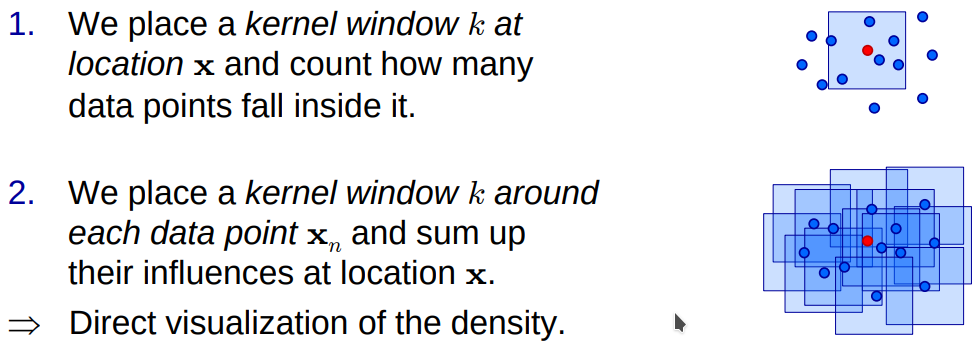
\includegraphics[width=.5\textwidth]{kernel_methods_interpretation}
    \end{figure}

    $\Rightarrow$ discontinuities at cube boundaries $\Rightarrow$ choose smoother kernel function...
    \item Gaussian kernel
    \begin{itemize}
      \item $k$ is now the normal distribution
      \[
        k(x - x_n) = \mathcal{N}(x_n | x, h^2)
      \]
      , with the center of the hypercube as $\mu$ and the width of the hypercube as $\sigma$. The volume $V$ is 1 in this case, as the normal distribution is a normalized pdf.

    \end{itemize}
    \item width $h$ acts as smoothing factor $->$ larger $h$ leads to more smoothing
  \end{itemize}
  \item \textbf{K-Nearest Neighbor}
  \begin{itemize}
    \item fixed $K$, determine $V$
    \item increase $V$ until the $K$ next data points are found
    \item position hypersphere with center-point $x$ and let it grow to volume $V*$ that includes $K$ of the $N$ given data points:
    \[
      p(x) \approx \frac{K}{NV*}
    \]
    \item K-nearest neighbor classification: lecture 3, page 53
  \end{itemize}
\end{itemize}

\subsection{Mixture distributions}

\begin{itemize}
  \item single parametric distribution often not sufficient
  \item mixture of Gaussians
  \begin{itemize}
    \item sum of $M$ individual normal distributions
    \[
      p(x|\theta) = \sum_{j=1}^M p(x|\theta_j)p(j)
    \]

    with \emph{mixture weights} $p(j)$:
    \[
      p(j) = \pi_j \quad \text{and} \quad \sum_j \pi_j = 1
    \]
    \item the mixture density integrates to 1
    \item again, we try to find a maximum likelihood estimate
    \begin{itemize}
      \item there is no direct analytical solution
      \item optimizing one Gaussian depends on all other Gaussians
      \item see lecture 4, page 45 for more details
    \end{itemize}
    \item alternative way needed for ML estimation
    \begin{itemize}
      \item either assume, that we know for each data point $x_n$ by which component it was created. Then, we could easily estimate the shape of the mixture components
      \item or assume, that we know the shape of the mixture components. Then, we could easily estimate for each data point $x_n$, the mixture component by which it was created
    \end{itemize}
  \end{itemize}
\end{itemize}

\subsubsection{Mixture component estimation}

\begin{itemize}
  \item hard assignment of data points to components by using k-means clustering
  \item expectation-maximization (EM) algorithm
  \begin{itemize}
    \item expectation step: softly assign data points to mixture components (calculate posterior of component, given the data point and the current parameters of the mixture components)
    \item maximization step: given the soft assignments, \\ (separately) re-estimate mixture components to maximize the likelihood
    \item technical advice for EM algorithm
    \begin{itemize}
      \item introduce regularization by enforcing a minimum width of the Gaussians. This avoids that mixtures collapse on single data points
      \item initialize EM parameters with means and standard deviations from clusters found by k-means (which converges much faster than EM)
    \end{itemize}
  \end{itemize}
\end{itemize}

Applications and summary of mixture models are shown in lecture 5, slide 39.

\section{Linear Discriminant Functions}

Before: model posterior probability by using Bayes' theorem.

Now: directly model decision boundary/ posterior probability.

\begin{itemize}
  \item 2-class decisions
  \begin{itemize}
    \item learn discriminant functions $y_i(x) \quad \forall i \in \{1, 2\}$ and decide for class $1$ if
    \[
      y_1(x) > y_2(x) \Leftrightarrow y_1(x) - y_2(x) > 0 \Leftrightarrow \mathbf{y(x)} > 0
    \]
    and for class 2 otherwise.
    \item focus on linear discriminant functions
    \[
      y(x) = w^\top x + w_0
    \]
    \item if data set can be perfectly classified by linear discriminant $->$ \emph{linearly separable}
    \item geometric interpretation
    \begin{figure}[H]
      \centering
      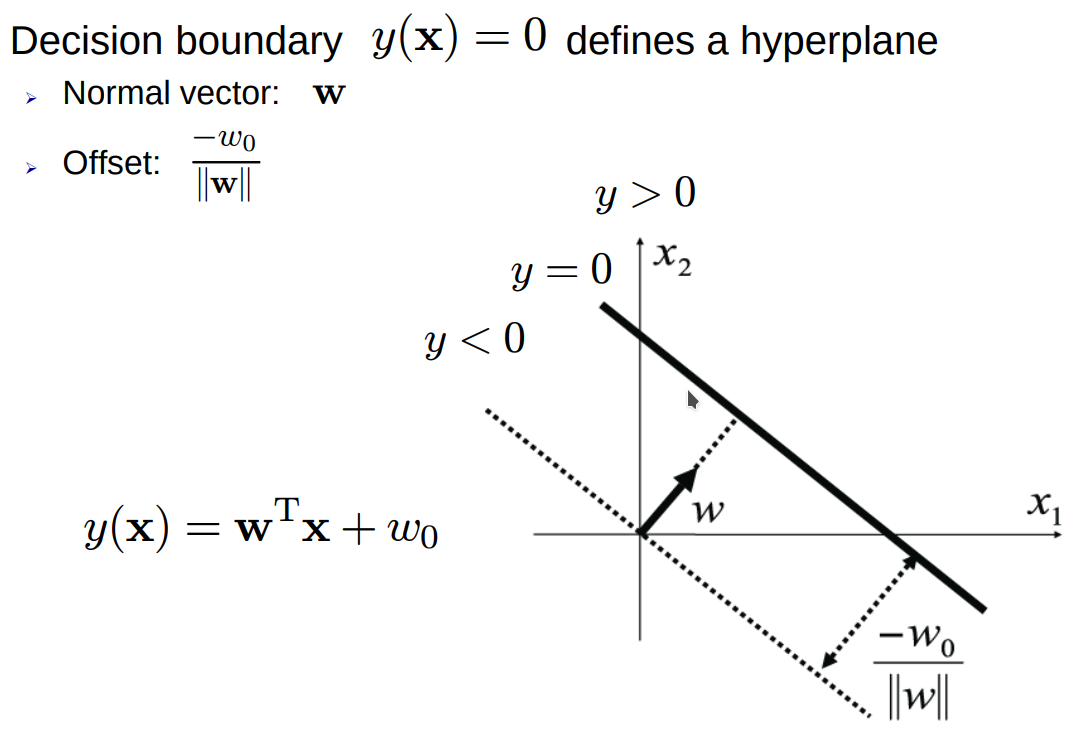
\includegraphics[width=.5\textwidth]{linear-discriminant-geometric}
    \end{figure}
    \item notation
    \begin{itemize}
      \item data points $x = (x_1, ..., x_D)^\top$ have $D$ dimensions
      \item $D$ weights + bias $->$ define $x_0 = 1$ to be constant
    \end{itemize}
  \end{itemize}
  \item extension to multi-class decisions
  \begin{itemize}
    \item one-vs-all
    \begin{itemize}
      \item for $k$ classes, train $k-1$ 1-vs-all classifiers
    \end{itemize}
    \item one-vs-one
    \begin{itemize}
      \item for $k$ classes, train $k(k-1)/2$ 1-vs-1 classifiers
    \end{itemize}
    \item problem: both methods lead to regions, where the decision is not clear
    \begin{itemize}
      \item e.g. for one-vs-all: what if multiple classifiers claim that it is their class?
    \end{itemize}
    \item solution: $k$-class discriminant
    \begin{itemize}
      \item use $k$ discriminant functions $y_k(x)$
      \item decide for class $k$ if
      \[
        y_k > y_j \quad \forall j\not = k
      \]
      \item hyperplanes are given by $(y_k-y_j)(x)$ for all $k \not = j$
    \end{itemize}
  \end{itemize}
\end{itemize}

\subsection{General Classification Problem}

\begin{itemize}
  \item given $k$ classes with corresponding classifiers $y_k$
  \item vector notation
  \[
    \mathbf{y(x) = \tilde{W}^\top x}
  \]
  , where $y(x)$ is a vector with $k$ entries (1 for each class)
  \item compare output to target value $t = (t_1, ..., t_k)^\top$
  \[
    y(x) - t
  \]
  \item for entire data set
  \[
    XW - T
  \]
  is a matrix of comparisons, where the rows correspond to data points and the columns correspond to classes
  \item find weights, which minimize some loss
  \begin{itemize}
    \item sum-of-squares error
    \[
      E(w) = \frac{1}{2} \sum_n \sum_k (w_k^\top x_n - t_{kn})^2.
    \]
    This has a closed-form solution (see lecture 6, page 27)
    \begin{itemize}
      \item problem: sensitive to outliers because of the squared error
    \end{itemize}
  \end{itemize}
\end{itemize}

\subsection{Generalized Linear Models}

\begin{itemize}
  \item introduce activation function $g$
  \[
    y(x) = g(w^\top x + w_0)
  \]
  \begin{itemize}
    \item for 2 classes: single-layer perceptron
    \item for $k$ classes: multi-class perceptron
  \end{itemize}
  \begin{itemize}
    \item sigmoid-function
    \begin{align*}
      p(C_1|x) &= \frac{p(x|C_1)p(C_1)}{p(x|C_1)p(C_1) + p(x|C_2)p(C_2)} \\
      \phantom{p(C_1|x)} &= \frac{1}{1 + \frac{p(x|C_2)p(C_2)}{p(x|C_1)p(C_1)}} \\
      \phantom{p(C_1|x)} &= \frac{1}{1 + \exp(-a)} =: g(a)
    \end{align*}
    \item softmax-function
    \begin{align*}
      p(C_k|x) &= \frac{p(x|C_k)p(C_k)}{\sum_j p(x|C_j)p(C_j)} \\
      \phantom{p(C_k|x)} &= \frac{\exp(a_k)}{\sum_j \exp(a_j)} =: g(a)
    \end{align*}
    \item both functions above allow us to interpret the $y(x)$ as posterior probabilities
    \item advantages
    \begin{itemize}
      \item helps limiting the effects of outliers ($g$ is bounded between 0 and 1 and therefore outputs cannot grow arbitrarily large)
      \item probabilistic interpretation
    \end{itemize}
    \item disadvantages
    \begin{itemize}
      \item in general, no closed-form analytical solution for least squares $->$ need to use iterative methods
    \end{itemize}
  \end{itemize}
  \item non-linear decision boundaries
  \begin{itemize}
    \item a single-layer perceptron with a non-linear activation function still has a linear decision boundary because the input features are linear
    \item solution: use multiple layers: the output of a single layer corresponds to $k$ linear decision boundaries. The next layer therefore combines multiple linear decision boundaries, which leads to non-linear decision boundaries
    \item in general, transform inputs $x$ with non-linear basis functions $\phi_j$
    \[
      y_k(x) = \sum_j w_{kj}\phi_j(x) + w_{k0}
    \]
    \begin{itemize}
      \item for multi-layer perceptrons, e.g. in the second layer, $\phi$ would be the function which is calculated by the first layer
    \end{itemize}
  \end{itemize}
\end{itemize}

\subsection{Gradient Descent}

\begin{itemize}
  \item iterative minimization
  \item in iteration $\tau + 1$, update weights by
  \[
    w_{kj}^{(\tau + 1)} = w_{kj}^{(\tau)} - \eta \frac{\partial E(w)}{\partial w_{kj}}
  \]
  \item strategies
  \begin{itemize}
    \item batch learning: compute gradient based on all training data
    \item sequential learning: compute gradient based on single data point at a time
  \end{itemize}
  \item delta-rule: when not using an activation function, the update is just the input data point, weighted by the classification error (lecture 6, page 48)
\end{itemize}

\subsection{Summary Linear Models}

\begin{figure}[H]
  \centering
  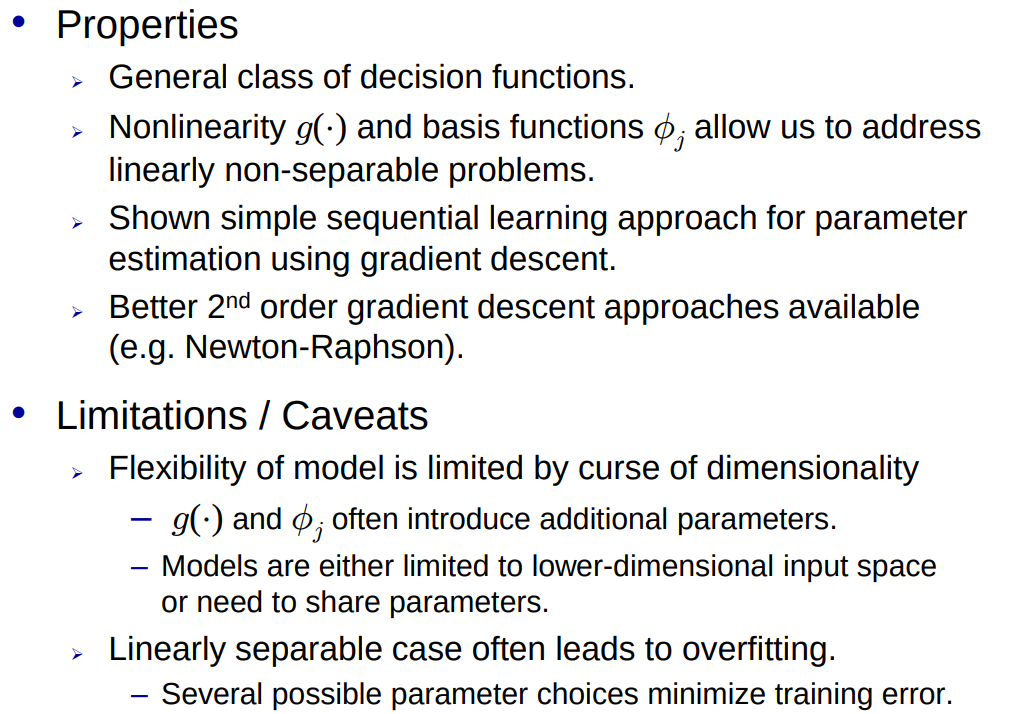
\includegraphics[width=.5\textwidth]{generalized_linear_discriminants_summary}
\end{figure}

\subsection{Logistic Regression}

\begin{itemize}
  \item model:
  \[
    p(C_1|\phi) = \sigma(w^\top \phi) = 1 - p(C_2|\phi)
  \]
  \item advantages over generative model
  \begin{itemize}
    \item number of parameters for $M$ dimensional data
    \begin{itemize}
      \item logistic regression: only weights $->$ one for each dimension of the input $->$ $M$ parameters
      \item generative Gaussian: for each class, we need one mean per dimension + the covariances $->$ $M(M+3)+1$ parameters
    \end{itemize}
  \end{itemize}
  \item maximum likelihood
  \begin{itemize}
    \item likelihood of the training data is given by
    \[
      p(t|w) = \prod_n y_n^{t_n}(1-y_n)^{1-t_n}
    \]
    \item error function is given by the negative log-likelihood (cross-entropy)
    \[
      E(w) = - \ln p(t|w)
    \]
    \item derivative of sigmoid with regard to weights:
    \begin{align*}
      y_n &= \sigma(w^\top \phi_n) \\
      \frac{\partial y_n}{\partial w} = y_n(1-y_n)\phi_n
    \end{align*}
    \item using the sigmoid activation function again leads to the delta-rule for gradient descent
  \end{itemize}
  \item Second-order Newton-Raphson gradient descent
  \begin{itemize}
    \item lecture 7, page 40
    \item more efficient than standard gradient descent
    \item closed-form solution for sum-of-squares error function (least-squares estimation)
    \item iterative for cross-entropy error function
  \end{itemize}
\end{itemize}

\subsection{Summary Logistic Regression}

\begin{figure}[H]
  \centering
  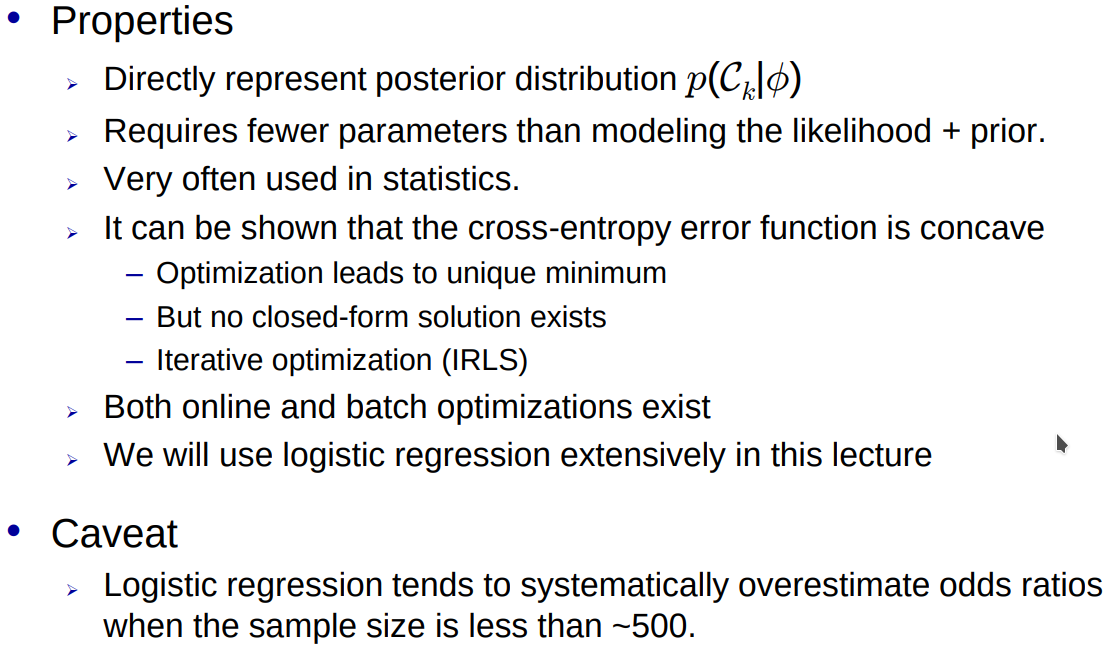
\includegraphics[width=.5\textwidth]{logistic_regression_summary}
\end{figure}

\subsection{Softmax Regression}

\begin{itemize}
  \item multi-class generalization of logistic regression
  \item cross-entropy function basically the same but with more than 2 labels
  \item again no closed-form solution for minimization of error function $->$ gradient descent
\end{itemize}

\subsection{Error Function Discussion}

See lecture 7, page 50.

\section{Support Vector Machines}

\subsection{Cross-validation}

\begin{itemize}
  \item $k$-fold cross-validation
  \begin{itemize}
    \item split data into 5 parts: train on 4 and test on the 5th
    \item do for all splits
    \item choose model with minimal validation error
  \end{itemize}
\end{itemize}

\subsection{Support Vector Machines}

For linearly separable data, many classifiers (decision boundaries) exist to separate the data.

\begin{itemize}
  \item question: how to select the linear classifier with the best generalization performance?
  \item answer
  \begin{itemize}
    \item choose classifier, which leaves maximal "safety room" for future data points
    \item maximize margin between positive and negative data points
  \end{itemize}
  \item linear decision boundary
  \begin{figure}[H]
    \centering
    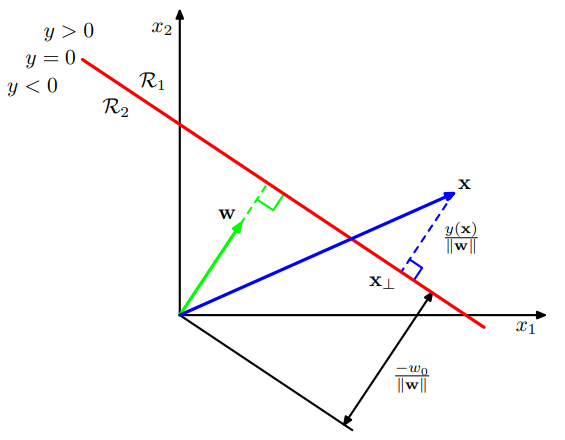
\includegraphics[width=.7\textwidth]{linear-discriminant-geometric2}
  \end{figure}
  \item margin of hyperplane
  \begin{itemize}
    \item let $d_-, d_+$ be the distance from the hyperplane to the nearest negative/ positive training sample, respectively
    \item choose weights $w$ such that
    \[
      d_- = d_+ = \frac{1}{||w||},
    \]
    or, in other words:
    \begin{align*}
      \exists n: \quad w^\top x_n + b &= 1 \\
      \exists n: \quad w^\top x_n + b &= -1
    \end{align*}
    \item this leads to a hyperplane with
    \[
      t_n (w^\top x_n + b) \geq 1 \quad \forall n,
    \]

    where $t_n$ is the true class of sample $x_n$.
  \end{itemize}
\end{itemize}














\end{document}
